%%%%%%%%%%%%%%%%%%%%%%%%%%%%%%%%%%%%%%%%%
% Dinara Nikolaeva made minor edits (jan 2015)  to : 
% Masters/Doctoral Thesis 
% LaTeX Template
% Version 1.43 (17/5/14)
%
% This template has been downloaded from:
% http://www.LaTeXTemplates.com
%
% Original authors:
% Steven Gunn 
% http://users.ecs.soton.ac.uk/srg/softwaretools/document/templates/
% and
% Sunil Patel
% http://www.sunilpatel.co.uk/thesis-template/
% and
% Dinara Nikolaeva
% http://www.sunilpatel.co.uk/thesis-template/
%
% License:
% CC BY-NC-SA 3.0 (http://creativecommons.org/licenses/by-nc-sa/3.0/)
%
% Note:
% Make sure to edit document variables in the Thesis.cls file
%
%%%%%%%%%%%%%%%%%%%%%%%%%%%%%%%%%%%%%%%%%

%----------------------------------------------------------------------------------------
%	PACKAGES AND OTHER DOCUMENT CONFIGURATIONS
%----------------------------------------------------------------------------------------

\documentclass[11pt, oneside]{Thesis} % The default font size and one-sided printing (no margin offsets)

\graphicspath{{Pictures/}} % Specifies the directory where pictures are stored

% \usepackage[square, comma, sort&compress]{natbib} % Use the natbib reference package - read up on this to edit the reference style; if you want text (e.g. Smith et al., 2012) for the in-text references (instead of numbers), remove 'numbers' 
\usepackage[square,numbers]{natbib}

\hypersetup{urlcolor=blue, colorlinks=true} % Colors hyperlinks in blue - change to black if annoying


\title{HSE CS Masters thesis template} % BUT you should use use " \title{\ttitle} " here instead to define the thesis title ! 
% \ttitle is defined in the file Thesis.cls 

\begin{document}

\frontmatter % Use roman page numbering style (i, ii, iii, iv...) for the pre-content pages

\setstretch{1.3} % Line spacing of 1.3

% Define the page headers using the FancyHdr package and set up for one-sided printing
\fancyhead{} % Clears all page headers and footers
\rhead{\thepage} % Sets the right side header to show the page number
\lhead{} % Clears the left side page header

\pagestyle{fancy} % Finally, use the "fancy" page style to implement the FancyHdr headers

\newcommand{\HRule}{\rule{\linewidth}{0.5mm}} % New command to make the lines in the title page

% PDF meta-data
\hypersetup{pdftitle={\ttitle}}
\hypersetup{pdfsubject=\subjectname}
\hypersetup{pdfauthor=\authornames}
\hypersetup{pdfkeywords=\keywordnames}

%----------------------------------------------------------------------------------------
%	TITLE PAGE ENGLISH
%----------------------------------------------------------------------------------------

\begin{titlepage}
\begin{center}

\begin{minipage}{0.99\textwidth}
\begin{flushleft} \large

\includegraphics[width=8cm]{./Figures/logo_hse.jpg} % University/department logo - uncomment to place it
% \emph{Author:}\\
% \href{https://github.com/super-position}{\authornames} % Author name - remove the \href bracket to remove the link
\end{flushleft}
\end{minipage}

\textsc{\univname}\\[1.5cm] % University name
\textbf{\textit{\Large Faculty of witchcraft and wizardry}}\\[0.5cm] % Thesis type
% \textsc{\Large First Last-Name}\\[0.5cm] % Thesis type
\href{https://github.com/super-position}{\authornames} % Author name - remove the \href bracket to remove the link


\HRule \\[0.4cm] % Horizontal line
{\huge \bfseries \ttitle}\\[0.4cm] % Thesis title
\HRule \\[1.5cm] % Horizontal line

 
\textbf{Group} \underline{GROUP2019}

\large \textbf{}{Qualification paper – Master of Science Dissertation\\ Field of study 01.01.01 Linear Happiness}\\[0.3cm] % University requirement text
% A thesis submitted in fulfilment of the requirements\\ for the degree of \degreename

\textbf{}{Program: Dark Time Manipulation}\\[0.4cm]

% \deptname\\[2cm] % Research group name and department name
 %\groupname\\[2cm]
 
% \begin{minipage}{0.4\textwidth}
% \begin{flushleft} \large
% \emph{Author:}\\
% \href{https://github.com/super-position}{\authornames} % Author name - remove the \href bracket to remove the link
% \end{flushleft}
% \end{minipage}

\begin{minipage}{0.8\textwidth}
\begin{flushright} \large
\emph{Supervisor:} \\
\href{https://www.hse.ru/en/org/persons/22564953}{\supname} % Supervisor name - remove the \href bracket to remove the link  
\end{flushright}
\end{minipage}\\[6cm]

% 
\includegraphics[width=10cm]{./Figures/logo_hse.jpg} % University/department logo - uncomment to place it

{\large \today}\\[1cm] % Date

\vfill
\end{center}

\end{titlepage}

%----------------------------------------------------------------------------------------
%	DECLARATION PAGE
%	Your institution may give you a different text to place here
%----------------------------------------------------------------------------------------

\Declaration{

\addtocontents{toc}{\vspace{1em}} % Add a gap in the Contents, for aesthetics

I, \authornames, declare that this thesis titled, '\ttitle' and the work presented in it is my own. I confirm that this work submitted for assessment is my own and is
  expressed in my own words. Any uses made within it of the works of
  other authors in any form (e.g., ideas, equations, figures, text,
  tables, programs) are properly acknowledged at any point of their
  use. A list of the references employed is included.

%\begin{itemize} 
%\item[\tiny{$\blacksquare$}] This work was done wholly or mainly while in candidature for a research degree at this University.
%\item[\tiny{$\blacksquare$}] Where any part of this thesis has previously been submitted for a degree or any other qualification at %this University or any other institution, this has been clearly stated.
%\item[\tiny{$\blacksquare$}] Where I have consulted the published work of others, this is always clearly attributed.
%\item[\tiny{$\blacksquare$}] Where I have quoted from the work of others, the source is always given. With the exception of such %quotations, this thesis is entirely my own work.
%\item[\tiny{$\blacksquare$}] I have acknowledged all main sources of help.
%\item[\tiny{$\blacksquare$}] Where the thesis is based on work done by myself jointly with others, I have made clear exactly what %was done by others and what I have contributed myself.\\
%\end{itemize}
 \vspace{2cm} 
Signed:\\
\rule[1em]{25em}{0.5pt} % This prints a line for the signature
 
Date:\\ 
\rule[1em]{25em}{0.5pt} % This prints a line to write the date
}

\clearpage % Start a new page

%----------------------------------------------------------------------------------------
%	QUOTATION PAGE
%----------------------------------------------------------------------------------------

\pagestyle{empty} % No headers or footers for the following pages

\null\vfill % Add some space to move the quote down the page a bit

\textit{"Don't begin social contact with anyone, be engineer."}
\begin{flushright}
\href{http://www.vernon.eu/}{David Vernon}
\end{flushright}

\textit{"If I have seen further than others, it is by standing upon the shoulders of giants."}
\begin{flushright}
\href{https://en.wikipedia.org/wiki/Isaac_Newton}{Isaac Newton}
\end{flushright}

\vfill\vfill\vfill\vfill\vfill\vfill\null % Add some space at the bottom to position the quote just right

\clearpage % Start a new page

%----------------------------------------------------------------------------------------
%	ABSTRACT PAGE English
%----------------------------------------------------------------------------------------

\addtotoc{Abstract} % Add the "Abstract" page entry to the Contents

%\abstract{\addtocontents{toc}{\vspace{1em}} % Add a gap in the Contents, for aesthetics

 {\huge{\textit{Abstract}} \par}{\addtocontents{toc}{\vspace{1em}} 

\par The abstract should be approximately 200 words long. It normally takes at least ten revisions to achieve a good abstract.

\par The abstract should be written after the thesis has been completed.

\begin{itemize}
    \item What is the subject matter of the thesis: what did you do?
    \item Motivation: why is it important?
    \item Significance: what contribution does the thesis make?
\end{itemize}

\par The page is kept centered vertically so can expand into the blank space above the title too.
\ldots
%

\clearpage % Start a new page

%----------------------------------------------------------------------------------------
%	ACKNOWLEDGEMENTS
%----------------------------------------------------------------------------------------

\setstretch{1.3} % Reset the line-spacing to 1.3 for body text (if it has changed)

\acknowledgements{\addtocontents{toc}{\vspace{1em}} % Add a gap in the Contents, for aesthetics

\par This project’s successful outcome was the result of a massive effort of the \href{https://en.wikipedia.org/wiki/Nuton}{Isaac Newton} and his team, with team members across Mathematics, Mechanical Engineering, Electrical Engineering, Computer Science, Business Management and Administration units. This work could not have been completed without their contribution to the project.

\par The \href{https://en.wikipedia.org/wiki/Stephen_Hawking}{Stephen Hawking} team was fortunate to have sponsors, supporters, press, who generously provided help and funding for this project, their support is hereby acknowledged and well appreciated. 

\par Additionally, we would like to thank \href{https://en.wikipedia.org/wiki/Albert_Einstein}{Albert Einstein} and \href{https://en.wikipedia.org/wiki/Nikola_Tesla}{Nikola Tesla} for their work.  
}
\clearpage % Start a new page

%----------------------------------------------------------------------------------------
%	LIST OF CONTENTS/FIGURES/TABLES PAGES
%----------------------------------------------------------------------------------------

\pagestyle{fancy} % The page style headers have been "empty" all this time, now use the "fancy" headers as defined before to bring them back

\lhead{\emph{Contents}} % Set the left side page header to "Contents"
\tableofcontents % Write out the Table of Contents

\lhead{\emph{List of Figures}} % Set the left side page header to "List of Figures"
\listoffigures % Write out the List of Figures

\lhead{\emph{List of Tables}} % Set the left side page header to "List of Tables"
\listoftables % Write out the List of Tables

%----------------------------------------------------------------------------------------
%	ABBREVIATIONS
%----------------------------------------------------------------------------------------

\clearpage % Start a new page

\setstretch{1.5} % Set the line spacing to 1.5, this makes the following tables easier to read

\lhead{\emph{Abbreviations}} % Set the left side page header to "Abbreviations"
\listofsymbols{ll} % Include a list of Abbreviations (a table of two columns)
{

\textbf{MAG} & \textbf{M}astering \textbf{A}t \textbf{G}aming \\
\textbf{MG} & \textbf{M}astering \textbf{G}ravity \\

%\textbf{Acronym} & \textbf{W}hat (it) \textbf{S}tands \textbf{F}or \\
}

%----------------------------------------------------------------------------------------
%	PHYSICAL CONSTANTS/OTHER DEFINITIONS
%----------------------------------------------------------------------------------------

%\clearpage % Start a new page

%\lhead{\emph{Physical Constants}} % Set the left side page header to "Physical Constants"

%\listofconstants{lrcl} % Include a list of Physical Constants (a four column table)
%{
%Speed of Light & $c$ & $=$ & $2.997\ 924\ 58\times10^{8}\ \mbox{ms}^{-\mbox{s}}$ (exact)\\

%% Constant Name & Symbol & = & Constant Value (with units) \\
%}

%----------------------------------------------------------------------------------------
%	SYMBOLS
%----------------------------------------------------------------------------------------

\clearpage % Start a new page

\lhead{\emph{Symbols}} % Set the left side page header to "Symbols"

\listofnomenclature{lll} % Include a list of Symbols (a three column table)
{
$a$ & distance & m \\
$P$ & power & W (Js$^{-1}$) \\
% Symbol & Name & Unit \\

& & \\ % Gap to separate the Roman symbols from the Greek

$\omega$ & angular frequency & rads$^{-1}$ \\
% Symbol & Name & Unit \\
}

%----------------------------------------------------------------------------------------
%	DEDICATION
%----------------------------------------------------------------------------------------

\setstretch{1.3} % Return the line spacing back to 1.3

\pagestyle{empty} % Page style needs to be empty for this page

\dedicatory{First of all, I would like to express my deep gratitude to Prof. \href{https://www.lesswrong.com/}{Quirrell}, who supervised and guided my research work. From the very beginning, he trusted and motivated me to strive for the highest goals. While I was struggling with some hard research problems, he encouraged me to continue, stay focused, be accurate, and showed me the big picture. Second, thanks to all people, who helped me gain a solid academic training. Without these people, I would never gain new knowledge and different perspectives to determine what is really going on. Furthermore, I want to thank \href{http://www.hpmor.com/}{Eliezer Yudkowsky}, with whom I have worked closely during this thesis. The cooperation with him was always constructive and meant a lot of fun for both of us. Special thanks deserve  \href{https://en.wikipedia.org/wiki/Arkady_and_Boris_Strugatsky}{Arkady Natanovich Strugatsky and Boris Natanovich Strugatsky} for proof-reading my master’s thesis. I know, it was not an easy task. Moreover, I would like to thank \href{https://en.wikipedia.org/wiki/Ready_Player_One}{Ernest Cline} for in-time comment about the testing chapter. Finally, and most deeply, I want to thank my big family and friends, grandparents and parents, whom I definitely saw too rarely during my time in Moscow. Without their endless support, love, and belief in me I would not have been able to accomplish this thesis. I am eternally grateful to them and dedicate this thesis to them.} % Dedication text

\addtocontents{toc}{\vspace{2em}} % Add a gap in the Contents, for aesthetics

%----------------------------------------------------------------------------------------
%	THESIS CONTENT - CHAPTERS
%----------------------------------------------------------------------------------------

\mainmatter % Begin numeric (1,2,3...) page numbering

\pagestyle{fancy} % Return the page headers back to the "fancy" style

% Include the chapters of the thesis as separate files from the Chapters folder
% Uncomment the lines as you write the chapters

% Chapter 1
\chapter{Introduction} % Main chapter title
\label{Chapter1} % For referencing the chapter elsewhere, use \ref{Chapter1} 
\lhead{Chapter 1. \emph{Introduction}} % This is for the header on each page - perhaps a shortened title
%----------------------------------------------------------------------------------------

\par This is general template for those wizards, who rose above and beyond Word. From now on, they can manipulate the reality and matter with new so advanced tool \LaTeX{}.

\par  Blown Away By Magic!

%----------------------------------------------------------------------------------------
\section{Motivation}
%----------------------------------------------------------------------------------------

\par 

\par 

\par 

%----------------------------------------------------------------------------------------
\subsection{Abstract}
%----------------------------------------------------------------------------------------

\par Figure \ref{fig:phd-abstract.png} see more \href{https://phdcomics.com/comics/archive_print.php?comicid=1121}{in}.
% https://phdcomics.com/comics/archive_print.php?comicid=1121

\begin{figure}[H]
    \centering
    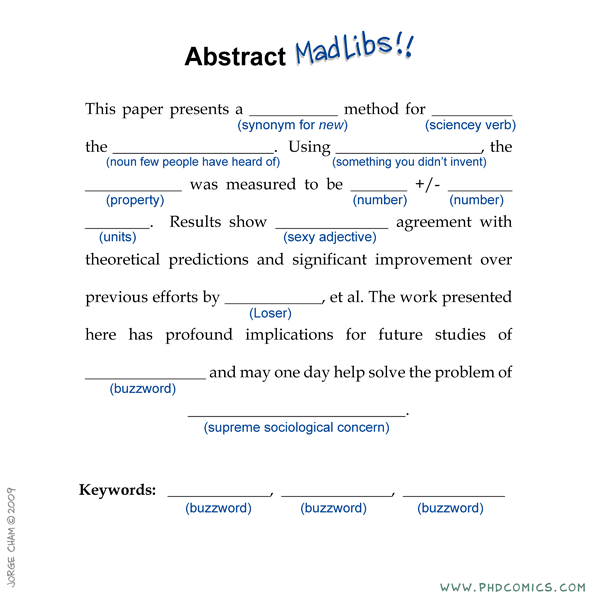
\includegraphics[scale=0.9]{Figures/phd-abstract.png}
    %\rule{35em}{0.5pt}
    \caption[Abstract]{\href{https://phdcomics.com/comics/archive_print.php?comicid=1121}{Abstract}}
    \label{fig:phd-abstract.png}
\end{figure}

%----------------------------------------------------------------------------------------
\subsection{Outline}
%----------------------------------------------------------------------------------------

\par Look other your outline Figure \ref{fig:phd-outline.png} see more \href{http://phdcomics.com/comics/archive.php?comicid=715}{link}.
% http://phdcomics.com/comics/archive.php?comicid=715

\begin{figure}[H]
    \centering
    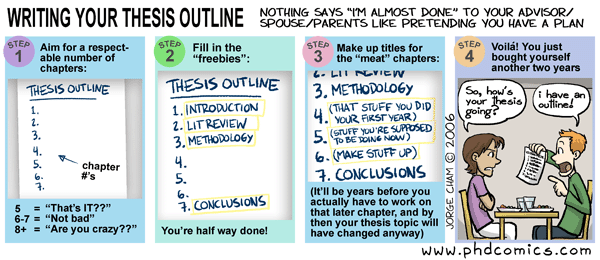
\includegraphics[scale=0.9]{Figures/phd-outline.png}
    %\rule{35em}{0.5pt}
    \caption[Outline]{\href{http://phdcomics.com/comics/archive.php?comicid=715}{Outline}}
    \label{fig:phd-outline.png}
\end{figure}

%----------------------------------------------------------------------------------------
\section{Background}
%----------------------------------------------------------------------------------------



\par 

\par 

%----------------------------------------------------------------------------------------
\subsection{Typical Structure of a Thesis}
%----------------------------------------------------------------------------------------

\begin{itemize}
    \item Title Page (Figure \ref{fig:phd-title.png})
    \item Specific title of the thesis (e.g. “Multi-stage Learning in Biomimetic Search and Rescue Robots”)
    \item General Title (i.e. “Final Year Project Report”)
\begin{figure}[H]
    \centering
    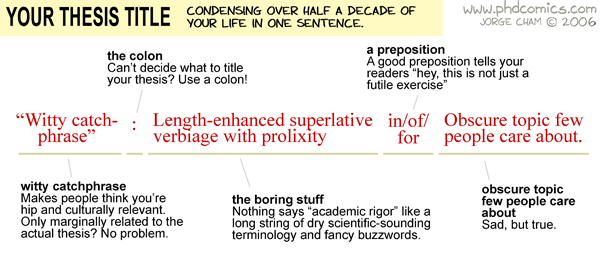
\includegraphics[scale=0.9]{Figures/phd-title.png}
    %\rule{35em}{0.5pt}
    \caption[Title]{\href{http://phdcomics.com/comics/archive_print.php?comicid=718}{Title}}
    \label{fig:phd-title.png}
\end{figure}

    \item Degree (e.g. Ph.D., M.Sc., B. Sc.)
    \item Author (name and student identification number)
    \item Institution 
    \item Supervisor
    \item Date
    \item Table of Contents
    \item Chapters
    \item Sections
    \item Acknowledgements (Help from friends, colleagues, and staff. Support from sponsor... Support from Parents, etc... )
     \item Chapter 1. Introduction & Overview
    \item Chapter 2. Literature Survey
    \item Chapter 3. Theoretical Foundations: Background Material
    \item Chapter 4. Formal Model: Theoretical Development (use additional chapters if necessary)
    \item Chapter 5. Algorithmic Considerations
    \item Chapter 6. Implementation Issues
    \item Chapter 7. Evaluation
    \item Chapter 8. Discussion and Critical Appraisal
    \item References
    \item Appendices
    \item Key Software listings, Code, Diagrams
    \item Mechanical schematics
    \item Mathematical proofs
\end{itemize}

%----------------------------------------------------------------------------------------
\subsection{Items}
%----------------------------------------------------------------------------------------

\par 

\begin{enumerate}
    \item One 
    \item Two
    \item 
    \item 
    \item 
    \item 
    \item 
\end{enumerate}

\begin{itemize}
    \item 1
    \item 2
    \item 
    \item 
    \item 
    \item 
    \item 
    \item 
\end{itemize}

\par 

\par 

%----------------------------------------------------------------------------------------
\section{Problem}
%----------------------------------------------------------------------------------------

\par 

%----------------------------------------------------------------------------------------
\section{Goals}
%----------------------------------------------------------------------------------------

\par 

%----------------------------------------------------------------------------------------
\section{Objectives}
%----------------------------------------------------------------------------------------

\par 

%----------------------------------------------------------------------------------------
\section{Contributions}
%----------------------------------------------------------------------------------------

\par 

%----------------------------------------------------------------------------------------
\section{Future goals}
%----------------------------------------------------------------------------------------

\par 

\par 

%----------------------------------------------------------------------------------------
\section{Outline}
%----------------------------------------------------------------------------------------

\par We will preside this thesis in a following structure \cite{David-Vernon}, \cite{David-Vernon1}:
\begin{itemize}
\item Chapter 1: Introduction, Background, Motivation, Problem statement, Goals, Restrictions, Overview;
\item Chapter 2: Literature Survey and Background:  Research method, Methodology of Software Development, Literature review, Related Works
\item Chapter 3: Theoretical Foundations: Background Material, State of art, Theory on hardware, Architecture
\item Chapter 4: Protocol and systems(services and programs) used to build the system.
\item Chapter 5: Formal Model: Theoretical Development, Implementation / Use cases, Testing
\item Chapter 6: Algorithmic Considerations
\item Chapter 7: Implementation Issues, Results and Evaluation
\item Chapter 8: Discussion, Critical Appraisal, Conclusions
\item Chapter 9: Future Work 
\end{itemize}

%Chapter 1. Introduction & Overview
%Chapter 2. Literature Survey
%Chapter 3. Theoretical Foundations: Background Material
%Chapter 4. Formal Model: Theoretical Development (use additional chapters if necessary)
%Chapter 5. Algorithmic Considerations
%Chapter 6. Implementation Issues
%Chapter 7. Evaluation
%Chapter 8. Discussion & Critical Appraisal
%References
%Appendices
% Key Software listings
% Mechanical schematics
% Mathematical proofs
%----------------------------------------------------------------------------------------
%----------------------------------------------------------------------------------------


%Typical Structure of a Thesis
%Title Page
% Specific title of the thesis (e.g. “Multi-stage Learning in Biomimetic Search and Rescue Robots”)
% General Title (i.e. “Final Year Project Report”)
%% Degree (e.g. Ph.D., M.Sc., B. Sc.)
% Author (name and student identification number)
% Institution (i.e. University of Skövde)
% Supervisor
% Date
%Abstract
% What is the subject matter of the thesis: what did you do?
% Motivation: why is it important?
% Significance: what contribution does the thesis make?
% The abstract should be approximately 200 words long. It normally takes at least ten revisions to achieve a good abstract.
% The abstract should be written after the thesis has been completed.
%Table of Contents
% Chapters
% Sections
%Acknowledgements
% Help from friends, colleagues, and staff.
% Support from sponsor
% Support from Parents, etc
%Chapter 1. Introduction & Overview
%Chapter 2. Literature Survey
%Chapter 3. Theoretical Foundations: Background Material
%Chapter 4. Formal Model: Theoretical Development (use additional chapters if necessary)
%Chapter 5. Algorithmic Considerations
%Chapter 6. Implementation Issues
%Chapter 7. Evaluation
%Chapter 8. Discussion & Critical Appraisal
%References
%Appendices
% Key Software listings
% Mechanical schematics
% Mathematical proofs
% Chapter 2
\chapter{Background} % Main chapter title
\label{Chapter2} % For referencing the chapter elsewhere, use \ref{Chapter1} 
\lhead{Chapter 2. \emph{State of Art}} % This is for the header on each page - perhaps a shortened title

\par 

%----------------------------------------------------------------------------------------
\section{Business justification for your work}
%----------------------------------------------------------------------------------------

\par 

\par 

%----------------------------------------------------------------------------------------
\subsection{Market research}
%----------------------------------------------------------------------------------------

\par 

\par 

%----------------------------------------------------------------------------------------
\section{Research methods}
%----------------------------------------------------------------------------------------


\par There are different methodologies, which can be used in order to conduct a research. Most of the researches apply scientific method see Figure \ref{fig:sci-method.png} .


\begin{figure}[H]
    \centering
    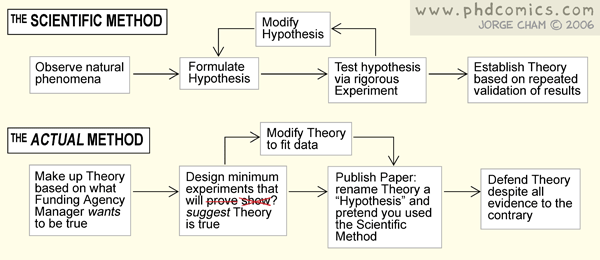
\includegraphics[scale=0.9]{Figures/sci-method.png}
    %\rule{35em}{0.5pt}
    \caption[Sci method]{Sci method}
    \label{fig:sci-method.png}
\end{figure}

\par Depending on the study, there are different techniques, which can be applied. In our case, during our project we did conduct few studies. In order to conduct our research we preside following steps: 

\begin{enumerate}
    \item Formulating the research problem;
    \item Extensive literature survey;
    \item Developing hypothesis;
    \item Preparing the research design;
    \item Determining sample design;
    \item Collecting data;
    \item Execution of the project and Implementation of the project;
    \item Analysis of data;
    \item Hypothesis testing;
    \item Generalization and interpretation;
    \item Preparation of the report / presentation of our results \cite{Research-Methodology-Methods-and-Techniques}.
\end{enumerate}

\par To be more precise, we had two major different studies in our hands. First one was about user experience of our application. Second one was about drawing conclusions and results from insulin sensor data. 

\par We used qualitative and quantitative research method approaches to our problems due to data type. So, we are going to explain research types and their differences (see Table \ref{table:2.1}) As well as, how we applied this methods.

\begin{table}[H]
\begin{tabular}{|l|l|}
\hline
\textbf{Qualitative} & \textbf{Quantitative} \\ \hline
\begin{tabular}[c]{@{}l@{}}Direct observation, Open-ended surveys, \\ Focus group, In-depth interviews,\\ Oral history, Participant observation, \\ Ethnographic observation, Content analysis.\\ In UX we could apply: Interviews \\ (directed, non-directed, ethnographic), \\ Surveys, Questionnaires, Usability Tests \\ (moderated, unmoderated, guerrilla), Card \\ sorting, Tree testing, A/B testing, \\ \\ \href{ https://www.oreilly.com/library/view/ux-research/9781491951286/ch04.html}{Persona development}, and \href{https://www.nngroup.com/articles/which-ux-research-methods/}{so on} ... \end{tabular} & \begin{tabular}[c]{@{}l@{}}Surveys, structured interviews, \\ observations, reviews of records / \\ numeric information:\\ Study population, Sampling, \\ Data collection, Data analysis,\\ \\  \href{https://libguides.usc.edu/writingguide/quantitative}{Statistical analysis}\end{tabular} \\ \hline
\begin{tabular}[c]{@{}l@{}}Primarily inductive process used to \\ formulate theory / hypotheses\end{tabular} & \begin{tabular}[c]{@{}l@{}}Primarily deductive process used to test \\ pre-specified concepts, constructs, and \\ hypotheses that make up a theory\end{tabular} \\ \hline
\begin{tabular}[c]{@{}l@{}}More subjective: describes a problem / \\ condition from the point of view of \\ those experiencing it\end{tabular} & \begin{tabular}[c]{@{}l@{}}More objective: provides observed \\ effects (interpreted by researchers) \\ of a program on a problem or condition\end{tabular} \\ \hline
Text-based, Descriptive data & Number-based, Numerical data \\ \hline
More in-depth information on a few cases & \begin{tabular}[c]{@{}l@{}}Less in-depth but more breadth of \\ information across a large number\\  of cases\end{tabular} \\ \hline
\begin{tabular}[c]{@{}l@{}}Unstructured or semi-structured \\ response options\end{tabular} & Fixed response options \\ \hline
No statistical tests & Statistical tests are used for analysis \\ \hline
\begin{tabular}[c]{@{}l@{}}Can be valid and reliable: \\ largely depends on skill \\ and rigor of the researcher\end{tabular} & \begin{tabular}[c]{@{}l@{}}Can be valid and reliable: \\ largely depends on the measurement \\ device or instrument used\end{tabular} \\ \hline
\begin{tabular}[c]{@{}l@{}}Time expenditure lighter on the \\ planning end and heavier \\ during the analysis phase\end{tabular} & \begin{tabular}[c]{@{}l@{}}Time expenditure heavier on the \\ planning phase and lighter on the \\ analysis phase\end{tabular} \\ \hline
Less generalizable & More generalizable \\ \hline
\end{tabular}
\caption{ \href{https://www.orau.gov/cdcynergy/soc2web/content/phase05/phase05_step03_deeper_qualitative_and_quantitative.htm}{Difference between quantitative and qualitative research methods applied}}
\label{table:2.1}
\end{table}

% https://www.publichealthnotes.com/differences-qualitative-quantitative-research/

%----------------------------------------------------------------------------------------
\subsection{Qualitative research - User Experience}
%----------------------------------------------------------------------------------------

\par We formulated a research problem as - smoothing user experience of glucose monitoring systems in Android devises.  While doing literature survey, we stumbled upon a study with a schematic diagram of the tailored mobile coaching system on diabetes management (see Figure \ref{fig:Schematic-diagram-of-the-tailored-mobile-coaching-system.jpg}). Their application design was developed for teaching about diabetes, however we realized - that we could tailor their solution a little and get an application for our case. As a result, we decided to formulate hypothesis, where we deduced, that an a diabetic Android application for controlling glucose level should combine functionality of: statistics on Iot devise, everyday dosages of insulin, diary on food and exercises, medical record keeper, notifications for regular and emergency situations. 

\par For a research design we used different methods. First, we conducted direct Interviews. Second, we used persona development method in order to identify categories of our main uses. Finally, we conducted usability tests for different prototypes. In each step, we changed the design by analyzing responses of our focus group. Furthermore , we challenged our hypothesis one more time. Next, we generalized and interpreted results, by which our first hypothesis were true. Therefor, we implemented final version of out design. 


\par Qualitative research method was helpful in our case because we were dealing with text-base data. As well as, we have to take into account, that it is more subjective data. Also, we (researchers) had to interpreted the data, which been collected from individuals with diabetes and their reaction to InsuPad with Android Application. Moreover, we were shoving images of different prototypes as well as different design of InsuPad itself. The final result of design of application is presented in next chapters.

%----------------------------------------------------------------------------------------
\section{Software Development Methodology}
%----------------------------------------------------------------------------------------

\par During development process we have to use a methodology in order to satisfy an end quality of the product. In our case, due to a limited time and specific requirements, which have to be implemented, we preseed with Dr. Winston W. Royce first described the Waterfall Model (see Figure \ref{fig:Unmodified-Waterfall-Development-Model.jpg}). This model with no iteration, sometimes called “stagewise”. However, in Dr. Winston W. Royce’s paper did not use the term “waterfall”, he described the process itself. It was firs mentioned in relation to developing software in “Managing the Development of Large Software Systems”. The model includes the following steps: System requirements, Software Requirements, Analysis, Program Design, Coding, Testing, and Operations. As we can see, an unmodified waterfall process does not allow iteration like: going back to previous steps. This places a heavy planning burden on the earlier steps, as well as risks management. Also, since each subsequent step cannot begin until the previous step ends, any delays in earlier steps cause delays to the later steps.

\begin{figure}[H]
    \centering
    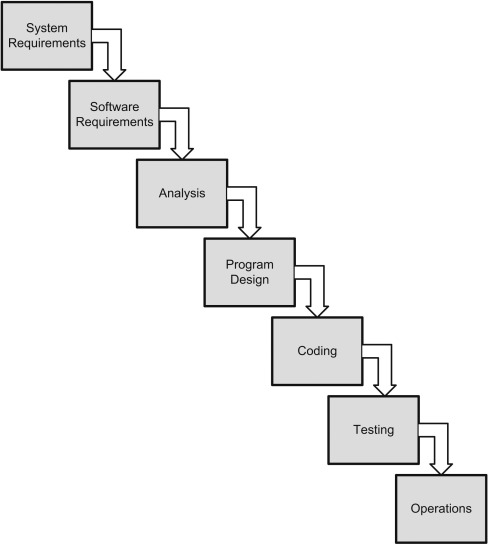
\includegraphics[scale=0.9]{Figures/Unmodified-Waterfall-Development-Model.jpg}
    %\rule{35em}{0.5pt}
    \caption[Unmodified-Waterfall-Development-Model]{Unmodified waterfall development model by Dr. Winston W. Royce. \cite{Unmodified-Waterfall-Development-Model}}
    \label{fig:Unmodified-Waterfall-Development-Model.jpg}
\end{figure}
% https://www.sciencedirect.com/topics/computer-science/waterfall-model

\par At the same time, we have the true demonstration of final thesis draft time-line in a Figure \ref{fig:thesis-word-count.png}. Of course  \href{https://www.lesswrong.com/posts/CPm5LTwHrvBJCa9h5/planning-fallacy}{planning fallacy} can be applied here.
% https://www.lesswrong.com/posts/CPm5LTwHrvBJCa9h5/planning-fallacy

\begin{figure}[H]
    \centering
    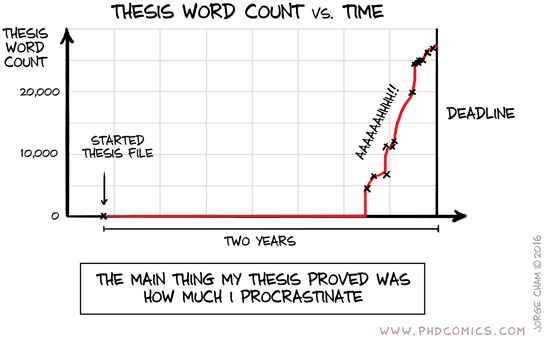
\includegraphics[scale=0.9]{Figures/thesis-word-count.png}
    %\rule{35em}{0.5pt}
    \caption[thesis-word-count]{\href{http://phdcomics.com/comics/archive_print.php?comicid=1915}{Thesis time-line}}
    \label{fig:thesis-word-count.png}
\end{figure}

%----------------------------------------------------------------------------------------
\section{Literature review}
%----------------------------------------------------------------------------------------
\pad In this section, we are going to look into researches of similar cases and similar applications. As well as, we are going to look into technologies and researches, which were used to make this product. 


%----------------------------------------------------------------------------------------
\subsection{}
%----------------------------------------------------------------------------------------


\par 

\par 

\par 

\par 

%C\item Chapter 1: Introduction, Background, Motivation, Problem statement, Goals, Restrictions, Overview;
%C\item Chapter 2: Literature Survey and Background:  Research method, Methodology of Software Development, Literature review, Related Works
%C\item Chapter 3: Theoretical Foundations: Background Material, State of art, Internet of Things, Theory on hardware, Serverless architecture
%C\item Chapter 4: Protocol and systems(services and programs) used to build the system.
%C\item Chapter 5: Formal Model: Theoretical Development, Implementation / Use cases, Testing
%C\item Chapter 6: Algorithmic Considerations
%C\item Chapter 7: Implementation Issues, Results and Evaluation
%C\item Chapter 8: Discussion, Critical Appraisal, Conclusions
%C\item Chapter 9: Future Work 

%Chapter 1. Introduction & Overview
%Chapter 2. Literature Survey
%Chapter 3. Theoretical Foundations: Background Material
%Chapter 4. Formal Model: Theoretical Development (use additional chapters if necessary)
%Chapter 5. Algorithmic Considerations
%Chapter 6. Implementation Issues
%Chapter 7. Evaluation
%Chapter 8. Discussion & Critical Appraisal
%References
%Appendices
% Key Software listings
% Mechanical schematics
% Mathematical proofs 
% Chapter 3

\chapter{State of the art} % Main chapter title

\label{Chapter3} % For referencing the chapter elsewhere, use \ref{Chapter1} 

\lhead{Chapter 3. \emph{State of the art}} % This is for the header on each page - perhaps a shortened title

%----------------------------------------------------------------------------------------
\par 

%----------------------------------------------------------------------------------------
\section{}
%----------------------------------------------------------------------------------------

\par 

\par

%----------------------------------------------------------------------------------------
\section{Architecture}
%----------------------------------------------------------------------------------------

\par 

\par 

%----------------------------------------------------------------------------------------
\subsection{}
%----------------------------------------------------------------------------------------
\par 

\par 

%----------------------------------------------------------------------------------------
\subsubsection{}
%----------------------------------------------------------------------------------------

\par 

%----------------------------------------------------------------------------------------
\section{}
%----------------------------------------------------------------------------------------

\par 

%----------------------------------------------------------------------------------------
\subsection{}
%----------------------------------------------------------------------------------------

\par 

\par 


\par 

\par 
%----------------------------------------------------------------------------------------
\subsection{}
%----------------------------------------------------------------------------------------

\par 

%-------------------------------------------------------------------------------------
\subsection{Application Architecture}
%-------------------------------------------------------------------------------------

\par 
%C\item Chapter 1: Introduction, Background, Motivation, Problem statement, Goals, Restrictions, Overview;
%C\item Chapter 2: Literature Survey and Background:  Research method, Methodology of Software Development, Literature review, Related Works
%C\item Chapter 3: Theoretical Foundations: Background Material, State of art, Internet of Things, Theory on hardware, Serverless architecture
%C\item Chapter 4: Protocol and systems(services and programs) used to build the system.
%C\item Chapter 5: Formal Model: Theoretical Development, Implementation / Use cases, Testing
%C\item Chapter 6: Algorithmic Considerations
%C\item Chapter 7: Implementation Issues, Results and Evaluation
%C\item Chapter 8: Discussion, Critical Appraisal, Conclusions
%C\item Chapter 9: Future Work 

%Chapter 1. Introduction & Overview
%Chapter 2. Literature Survey
%Chapter 3. Theoretical Foundations: Background Material
%Chapter 4. Formal Model: Theoretical Development (use additional chapters if necessary)
%Chapter 5. Algorithmic Considerations
%Chapter 6. Implementation Issues
%Chapter 7. Evaluation
%Chapter 8. Discussion & Critical Appraisal
%References
%Appendices
% Key Software listings
% Mechanical schematics
% Mathematical proofs
% Chapter 4

\chapter{Software and Hardware} % Main chapter title

\label{Chapter4} % For referencing the chapter elsewhere, use \ref{Chapter1} 

\lhead{Chapter 4. \emph{Software and Hardware}} % This is for the header on each page - perhaps a shortened title

\par 

%----------------------------------------------------------------------------------------
\section{}
%----------------------------------------------------------------------------------------

\par 

\par 

%----------------------------------------------------------------------------------------
\subsection{}
%----------------------------------------------------------------------------------------

\par 


%----------------------------------------------------------------------------------------
\section{}
%----------------------------------------------------------------------------------------


%----------------------------------------------------------------------------------------
\subsection{}
%----------------------------------------------------------------------------------------

%----------------------------------------------------------------------------------------
\subsection{}
%----------------------------------------------------------------------------------------

\par 

%C\item Chapter 1: Introduction, Background, Motivation, Problem statement, Goals, Restrictions, Overview;
%C\item Chapter 2: Literature Survey and Background:  Research method, Methodology of Software Development, Literature review, Related Works
%C\item Chapter 3: Theoretical Foundations: Background Material, State of art, Internet of Things, Theory on hardware, Serverless architecture
%C\item Chapter 4: Protocol and systems(services and programs) used to build the system.
%C\item Chapter 5: Formal Model: Theoretical Development, Implementation / Use cases, Testing
%C\item Chapter 6: Algorithmic Considerations
%C\item Chapter 7: Implementation Issues, Results and Evaluation
%C\item Chapter 8: Discussion, Critical Appraisal, Conclusions
%C\item Chapter 9: Future Work 

%Chapter 1. Introduction & Overview
%Chapter 2. Literature Survey
%Chapter 3. Theoretical Foundations: Background Material
%Chapter 4. Formal Model: Theoretical Development (use additional chapters if necessary)
%Chapter 5. Algorithmic Considerations
%Chapter 6. Implementation Issues
%Chapter 7. Evaluation
%Chapter 8. Discussion & Critical Appraisal
%References
%Appendices
% Key Software listings
% Mechanical schematics
% Mathematical proofs 
% Chapter 5

\chapter{Design and Implementation} % Main chapter title

\label{Chapter5} % For referencing the chapter elsewhere, use \ref{Chapter1} 

\lhead{Chapter 5. \emph{Design and Implementation}} % This is for the header on each page - perhaps a shortened title

\par 

\par 

% Chapter 5: Formal Model: Theoretical Development, Functional and Non-Functional Requirements, Implementation, Use cases, Testing

%----------------------------------------------------------------------------------------
\section{Functional Requirements}
%----------------------------------------------------------------------------------------

\par 

%----------------------------------------------------------------------------------------
\section{Non-Functional Requirements}
%----------------------------------------------------------------------------------------

\par 

%----------------------------------------------------------------------------------------
\section{Implementation}
%----------------------------------------------------------------------------------------

\par

%----------------------------------------------------------------------------------------
\section{Use cases}
%----------------------------------------------------------------------------------------

\par

%----------------------------------------------------------------------------------------
\section{Testing}
%----------------------------------------------------------------------------------------

\par

%----------------------------------------------------------------------------------------
\section{Results}
%----------------------------------------------------------------------------------------

\par For this section you will probably need some data to fit into other space - therefor just take a glance at your results and fit it into something - see figure \ref{fig:thesis-word-count.png}. 
% xkcd-python.png

\begin{figure}[H]
    \centering
    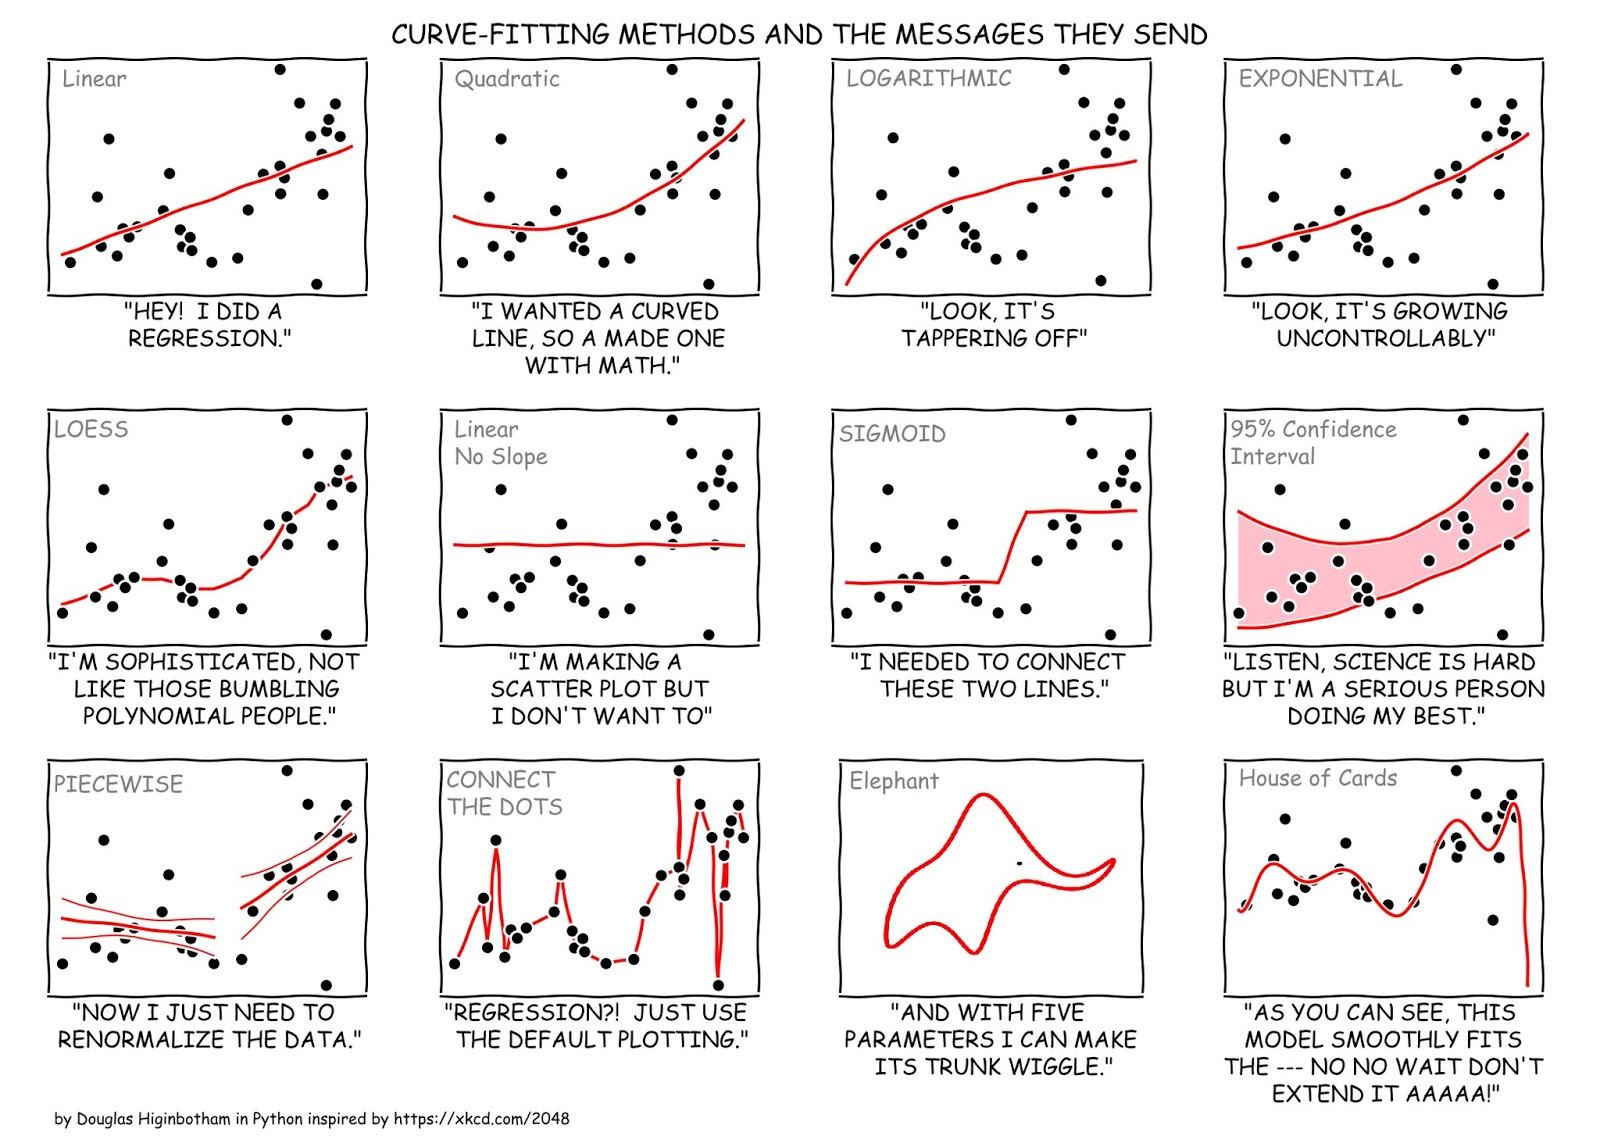
\includegraphics[scale=0.35]{Figures/xkcd-python.png}
    %\rule{35em}{0.5pt}
    \caption[Data fit]{Fit it}
    \label{fig:xkcd-python.png}
\end{figure}


%C\item Chapter 1: Introduction, Background, Motivation, Problem statement, Goals, Restrictions, Overview;
%C\item Chapter 2: Literature Survey and Background:  Research method, Methodology of Software Development, Literature review, Related Works
%C\item Chapter 3: Theoretical Foundations: Background Material, State of art, Internet of Things, Theory on hardware, Serverless architecture
%C\item Chapter 4: Protocol and systems(services and programs) used to build the system.
%C\item Chapter 5: Formal Model: Theoretical Development, Implementation / Use cases, Testing
%C\item Chapter 6: Algorithmic Considerations
%C\item Chapter 7: Implementation Issues, Results and Evaluation
%C\item Chapter 8: Discussion, Critical Appraisal, Conclusions
%C\item Chapter 9: Future Work 

%Chapter 1. Introduction & Overview
%Chapter 2. Literature Survey
%Chapter 3. Theoretical Foundations: Background Material
%Chapter 4. Formal Model: Theoretical Development (use additional chapters if necessary)
%Chapter 5. Algorithmic Considerations
%Chapter 6. Implementation Issues
%Chapter 7. Evaluation
%Chapter 8. Discussion & Critical Appraisal
%References
%Appendices
% Key Software listings
% Mechanical schematics
% Mathematical proofs 
% Chapter 6

\chapter{Algorithmic Considerations} % Main chapter title

\label{Chapter6} % For referencing the chapter elsewhere, use \ref{Chapter1} 

\lhead{Chapter 6. \emph{Algorithmic Considerations}} % This is for the header on each page - perhaps a shortened title

%C\item Chapter 1: Introduction, Background, Motivation, Problem statement, Goals, Restrictions, Overview;
%C\item Chapter 2: Literature Survey and Background:  Research method, Methodology of Software Development, Literature review, Related Works
%C\item Chapter 3: Theoretical Foundations: Background Material, State of art, Internet of Things, Theory on hardware, Serverless architecture
%C\item Chapter 4: Protocol and systems(services and programs) used to build the system.
%C\item Chapter 5: Formal Model: Theoretical Development, Implementation / Use cases, Testing
%C\item Chapter 6: Algorithmic Considerations
%C\item Chapter 7: Implementation Issues, Results and Evaluation
%C\item Chapter 8: Discussion, Critical Appraisal, Conclusions
%C\item Chapter 9: Future Work 

%Chapter 1. Introduction & Overview
%Chapter 2. Literature Survey
%Chapter 3. Theoretical Foundations: Background Material
%Chapter 4. Formal Model: Theoretical Development (use additional chapters if necessary)
%Chapter 5. Algorithmic Considerations
%Chapter 6. Implementation Issues
%Chapter 7. Evaluation
%Chapter 8. Discussion & Critical Appraisal
%References
%Appendices
% Key Software listings
% Mechanical schematics
% Mathematical proofs 
% Chapter 7

\chapter{Implementation Issues, Results and Evaluation} % Main chapter title

\label{Chapter7} % For referencing the chapter elsewhere, use \ref{Chapter1} 

\lhead{Chapter 7. \emph{Implementation Issues, Results and Evaluation}} % This is for the header on each page - perhaps a shortened title
%C\item Chapter 7: Implementation Issues, Results and Evaluation
%----------------------------------------------------------------------------------------
\section{1}
%----------------------------------------------------------------------------------------

\par 

%----------------------------------------------------------------------------------------
\subsection{1}
%----------------------------------------------------------------------------------------

\par 

%----------------------------------------------------------------------------------------
\section{1}
%----------------------------------------------------------------------------------------

\par 

%----------------------------------------------------------------------------------------
\section{1}
%----------------------------------------------------------------------------------------

\par 

%----------------------------------------------------------------------------------------
\subsection{1}
%----------------------------------------------------------------------------------------
%----------------------------------------------------------------------------------------

%C\item Chapter 1: Introduction, Background, Motivation, Problem statement, Goals, Restrictions, Overview;
%C\item Chapter 2: Literature Survey and Background:  Research method, Methodology of Software Development, Literature review, Related Works
%C\item Chapter 3: Theoretical Foundations: Background Material, State of art, Internet of Things, Theory on hardware, Serverless architecture
%C\item Chapter 4: Protocol and systems(services and programs) used to build the system.
%C\item Chapter 5: Formal Model: Theoretical Development, Implementation / Use cases, Testing
%C\item Chapter 6: Algorithmic Considerations
%C\item Chapter 7: Implementation Issues, Results and Evaluation
%C\item Chapter 8: Discussion, Critical Appraisal, Conclusions
%C\item Chapter 9: Future Work 

%Chapter 1. Introduction & Overview
%Chapter 2. Literature Survey
%Chapter 3. Theoretical Foundations: Background Material
%Chapter 4. Formal Model: Theoretical Development (use additional chapters if necessary)
%Chapter 5. Algorithmic Considerations
%Chapter 6. Implementation Issues
%Chapter 7. Evaluation
%Chapter 8. Discussion & Critical Appraisal
%References
%Appendices
% Key Software listings
% Mechanical schematics
% Mathematical proofs
% Chapter 8
\chapter{Discussion, Critical Appraisal, Conclusions} % Main chapter title
\label{Chapter8} % For referencing the chapter elsewhere, use \ref{Chapter8} 
\lhead{Chapter 8. \emph{Discussion, Critical Appraisal, Conclusions}} % This is for the header on each page - perhaps a shortened title
%----------------------------------------------------------------------------------------
%----------------------------------------------------------------------------------------
\section{1}
%----------------------------------------------------------------------------------------

\par 

%----------------------------------------------------------------------------------------
\subsection{1}
%----------------------------------------------------------------------------------------

\par 

%----------------------------------------------------------------------------------------
\section{1}
%----------------------------------------------------------------------------------------

\par 

%----------------------------------------------------------------------------------------
\section{1}
%----------------------------------------------------------------------------------------

\par 

%----------------------------------------------------------------------------------------
\subsection{1}
%----------------------------------------------------------------------------------------
%C\item Chapter 1: Introduction, Background, Motivation, Problem statement, Goals, Restrictions, Overview;
%C\item Chapter 2: Literature Survey and Background:  Research method, Methodology of Software Development, Literature review, Related Works
%C\item Chapter 3: Theoretical Foundations: Background Material, State of art, Internet of Things, Theory on hardware, Serverless architecture
%C\item Chapter 4: Protocol and systems(services and programs) used to build the system.
%C\item Chapter 5: Formal Model: Theoretical Development, Implementation / Use cases, Testing
%C\item Chapter 6: Algorithmic Considerations
%C\item Chapter 7: Implementation Issues, Results and Evaluation
%C\item Chapter 8: Discussion, Critical Appraisal, Conclusions
%C\item Chapter 9: Future Work 

%Chapter 1. Introduction & Overview
%Chapter 2. Literature Survey
%Chapter 3. Theoretical Foundations: Background Material
%Chapter 4. Formal Model: Theoretical Development (use additional chapters if necessary)
%Chapter 5. Algorithmic Considerations
%Chapter 6. Implementation Issues
%Chapter 7. Evaluation
%Chapter 8. Discussion & Critical Appraisal
%References
%Appendices
% Key Software listings
% Mechanical schematics
% Mathematical proofs
% Chapter 9
\chapter{Future Work} % Main chapter title
\label{Chapter9} % For referencing the chapter elsewhere, use \ref{Chapter1} 
\lhead{Chapter 9. \emph{Future Work}} % This is for the header on each page - perhaps a shortened title
%----------------------------------------------------------------------------------------
%----------------------------------------------------------------------------------------
\section{Additional Functionality}
%----------------------------------------------------------------------------------------
\par 
%----------------------------------------------------------------------------------------
\subsection{}
%----------------------------------------------------------------------------------------
\par 


\par 

%----------------------------------------------------------------------------------------
\subsection{}
%----------------------------------------------------------------------------------------

\par 

%----------------------------------------------------------------------------------------
\section{}
%----------------------------------------------------------------------------------------

\par 

\par 

%----------------------------------------------------------------------------------------
\section{}
%----------------------------------------------------------------------------------------

\par 




%C\item Chapter 1: Introduction, Background, Motivation, Problem statement, Goals, Restrictions, Overview;
%C\item Chapter 2: Literature Survey and Background:  Research method, Methodology of Software Development, Literature review, Related Works
%C\item Chapter 3: Theoretical Foundations: Background Material, State of art, Internet of Things, Theory on hardware, Serverless architecture
%C\item Chapter 4: Protocol and systems(services and programs) used to build the system.
%C\item Chapter 5: Formal Model: Theoretical Development, Implementation / Use cases, Testing
%C\item Chapter 6: Algorithmic Considerations
%C\item Chapter 7: Implementation Issues, Results and Evaluation
%C\item Chapter 8: Discussion, Critical Appraisal, Conclusions
%C\item Chapter 9: Future Work 

%Chapter 1. Introduction & Overview
%Chapter 2. Literature Survey
%Chapter 3. Theoretical Foundations: Background Material
%Chapter 4. Formal Model: Theoretical Development (use additional chapters if necessary)
%Chapter 5. Algorithmic Considerations
%Chapter 6. Implementation Issues
%Chapter 7. Evaluation
%Chapter 8. Discussion & Critical Appraisal
%References
%Appendices
% Key Software listings
% Mechanical schematics
% Mathematical proofs
 
%\input{Chapters/RusTitle.tex}
%\input{Chapters/RusAbstract.tex}

%----------------------------------------------------------------------------------------
%	THESIS CONTENT - APPENDICES
%----------------------------------------------------------------------------------------

\addtocontents{toc}{\vspace{2em}} % Add a gap in the Contents, for aesthetics

\appendix % Cue to tell LaTeX that the following 'chapters' are Appendices

% Include the appendices of the thesis as separate files from the Appendices folder
% Uncomment the lines as you write the Appendices

% Appendix A

\chapter{Appendix A} % Main appendix title

\label{AppendixA} % For referencing this appendix elsewhere, use \ref{AppendixA}

\lhead{Appendix A. \emph{User Interface of Application}} % This is for the header on each page - perhaps a shortened title

%% Appendix Template

\chapter{Appendix Title Here} % Main appendix title

\label{AppendixX} % Change X to a consecutive letter; for referencing this appendix elsewhere, use \ref{AppendixX}

\lhead{Appendix X. \emph{Appendix Title Here}} % Change X to a consecutive letter; this is for the header on each page - perhaps a shortened title

Write your Appendix content here.
%% Appendix Template

\chapter{Appendix Title Here} % Main appendix title

\label{AppendixX} % Change X to a consecutive letter; for referencing this appendix elsewhere, use \ref{AppendixX}

\lhead{Appendix X. \emph{Appendix Title Here}} % Change X to a consecutive letter; this is for the header on each page - perhaps a shortened title

Write your Appendix content here.

\addtocontents{toc}{\vspace{2em}} % Add a gap in the Contents, for aesthetics

\backmatter

%----------------------------------------------------------------------------------------
%	BIBLIOGRAPHY
%----------------------------------------------------------------------------------------

\label{Bibliography}

\lhead{\emph{Bibliography}} % Change the page header to say "Bibliography"

\bibliographystyle{apalike} % Use the "apalike" BibTeX style for formatting the Bibliography

\bibliography{Bibliography} % The references (bibliography) information are stored in the file named "Bibliography.bib"

\end{document}